\section{网页设计原理}
\subsection{软件及语言}
设计动态网页所用软件如下:
\begin{mylist1}
  \item Internet Information Services (IIS)。Web服务器软件,可以执行PHP语言。
  \item Dreamweaver CS6。它是一种有可视化编辑界面,用于制作并编辑网站的网页设计软件。
  \item PhpStudy for IIS 2014。它是一个集成IIS+PhpMyAdmin
  +PHP+MySQL于一体PHP调试环境程序集成包,。
  \item MySQLWorkbench。可视化MySQL数据库建模软件\cite{Ullman-418}。
\end{mylist1}

设计网页使用的语言如下:
\begin{mylist1}
\item 服务器端(后台)语言:PHP。
\item 浏览器端(前端)语言:HTML 、JQuery。JQuery是JavaScript的一种封装,是一个快速、简洁的JavaScript框架。
\item 数据库查询计语言:SQL。
\end{mylist1}
\subsection{数据库建立}
本文设计的动态网页用来管理汽车产品及其零部件。每一个汽车产品对应自己的零部件,分别建立汽车产品和汽车零部件表单。汽车产品表单各个字段如表\ref{tb:prd}所示,其中$prd\_id$为汽车产品表的主键。
\begin{table}[H]
	\setlength{\abovecaptionskip}{-10pt}   
	\setlength{\belowcaptionskip}{0pt}   %这2行是为了使表标题与表格距离适当
	\caption{汽车产品表}
	\begin{center}
		\begin{tabularx}{\textwidth}{YY}
			\toprule  
			字段 & 示例  \\ 
			\midrule 
			$prd\_id$ & 2  \\ 
			$prd\_num$ & P16 \\ 
			$prd\_style$ & 	POLO 1.4L \\ 
			$prd\_name$ & 全新POLO2016款 自动风尚版 \\
			$prd\_manf$ & 上海大众汽车 \\
			$prd\_area$ & 上海嘉定 \\
			$prd\_price$ & 80000 \\
			\bottomrule
		\end{tabularx} 
	\end{center}
	\label{tb:prd}
\end{table}

零件表如表\ref{tb:prt}所示,其中的	$prt\_id$为零部件表的主键,而$car\_prod\_prd\_id $则为外键即汽车产品在零件表中的体现。
\begin{table}[H]
	\setlength{\abovecaptionskip}{-10pt}   
	\setlength{\belowcaptionskip}{0pt}   %这2行是为了使表标题与表格距离适当
	\caption{零部件表}
	\begin{center}
		\begin{tabularx}{\textwidth}{YY}
			\toprule  
			字段 & 示例  \\ 
			\midrule 
			$prt\_id$ & 26  \\ 
			$prt\_num$ & PL04 \\ 
			$car\_prod\_prd\_id $ & 2 \\ 
			$prt\_name$ & 上海大众POLO自动变速器 \\
			$prt\_manf$ & Aisin-AW公司车 \\
			$prt\_manfAdr$ & 日本 \\
			$prt\_price$ & 4000 \\
			\bottomrule
		\end{tabularx} 
	\end{center}
	\label{tb:prt}
\end{table}

本文网页的各个功能,只有已注册用户才能使用,所以本文还设计了用户信息表\ref{tb:user}。其中的密码($r\_pass$)字段值以密文存储。
\begin{table}[H]
	\setlength{\abovecaptionskip}{-10pt}   
	\setlength{\belowcaptionskip}{0pt}   %这2行是为了使表标题与表格距离适当
	\caption{用户信息表}
	\begin{center}
		\begin{tabularx}{\textwidth}{YY}
			\toprule  
			字段 & 示例  \\ 
			\midrule 
			$r\_id$ & 1 \\ 
			$r\_name$ & admin \\ 
			$r\_pass$ & 21232f297a57a5a743894a0e4a801fc3 \\ 
			$r\_date$ & 2016-12-17 \\
			\bottomrule
		\end{tabularx} 
	\end{center}
	\label{tb:user}
\end{table}

按照上述思路,在MySQLWorkbench中建立由汽车产品表(car\_prod)、零部件表(car\_part)和用户表(reg)组成的数据库。数据库模型如图\ref{fig:cardb}所示,一个汽车产品对应多个零件(即一对多关系数据库)。
\begin{figure}[H]
\centering
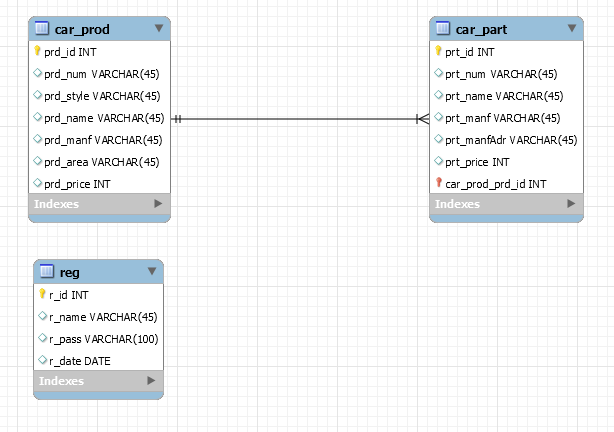
\includegraphics[width=0.9\linewidth]{figure/cardb}
\caption{汽车PDM数据库}
\label{fig:cardb}
\end{figure}
\subsection{动态网页结构}
本文设计的动态网页结构图\ref{fig:webStruk}所示。用户通过客户端浏览器(比如谷歌浏览器)向服务器(比如IIS)发出请求,可以实现对MySQL数据库中的数据进行操作(比如信息查询、删除、修改、添加和BOM表显示等)。
\begin{figure}[H]
\centering
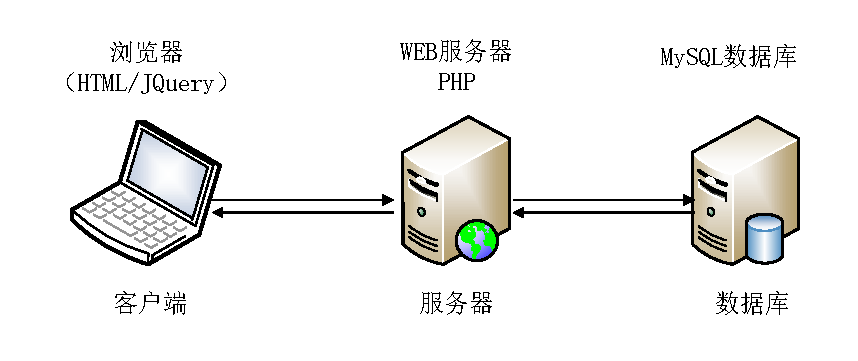
\includegraphics[width=1\linewidth]{figure/webStruk}
\caption{汽车PDM动态网页结构}
\label{fig:webStruk}
\end{figure}

\par~~~~~~~~~~

 网页在谷歌浏览器中的显示效果如图\ref{fig:index}所示。
\begin{figure}[H]
\centering
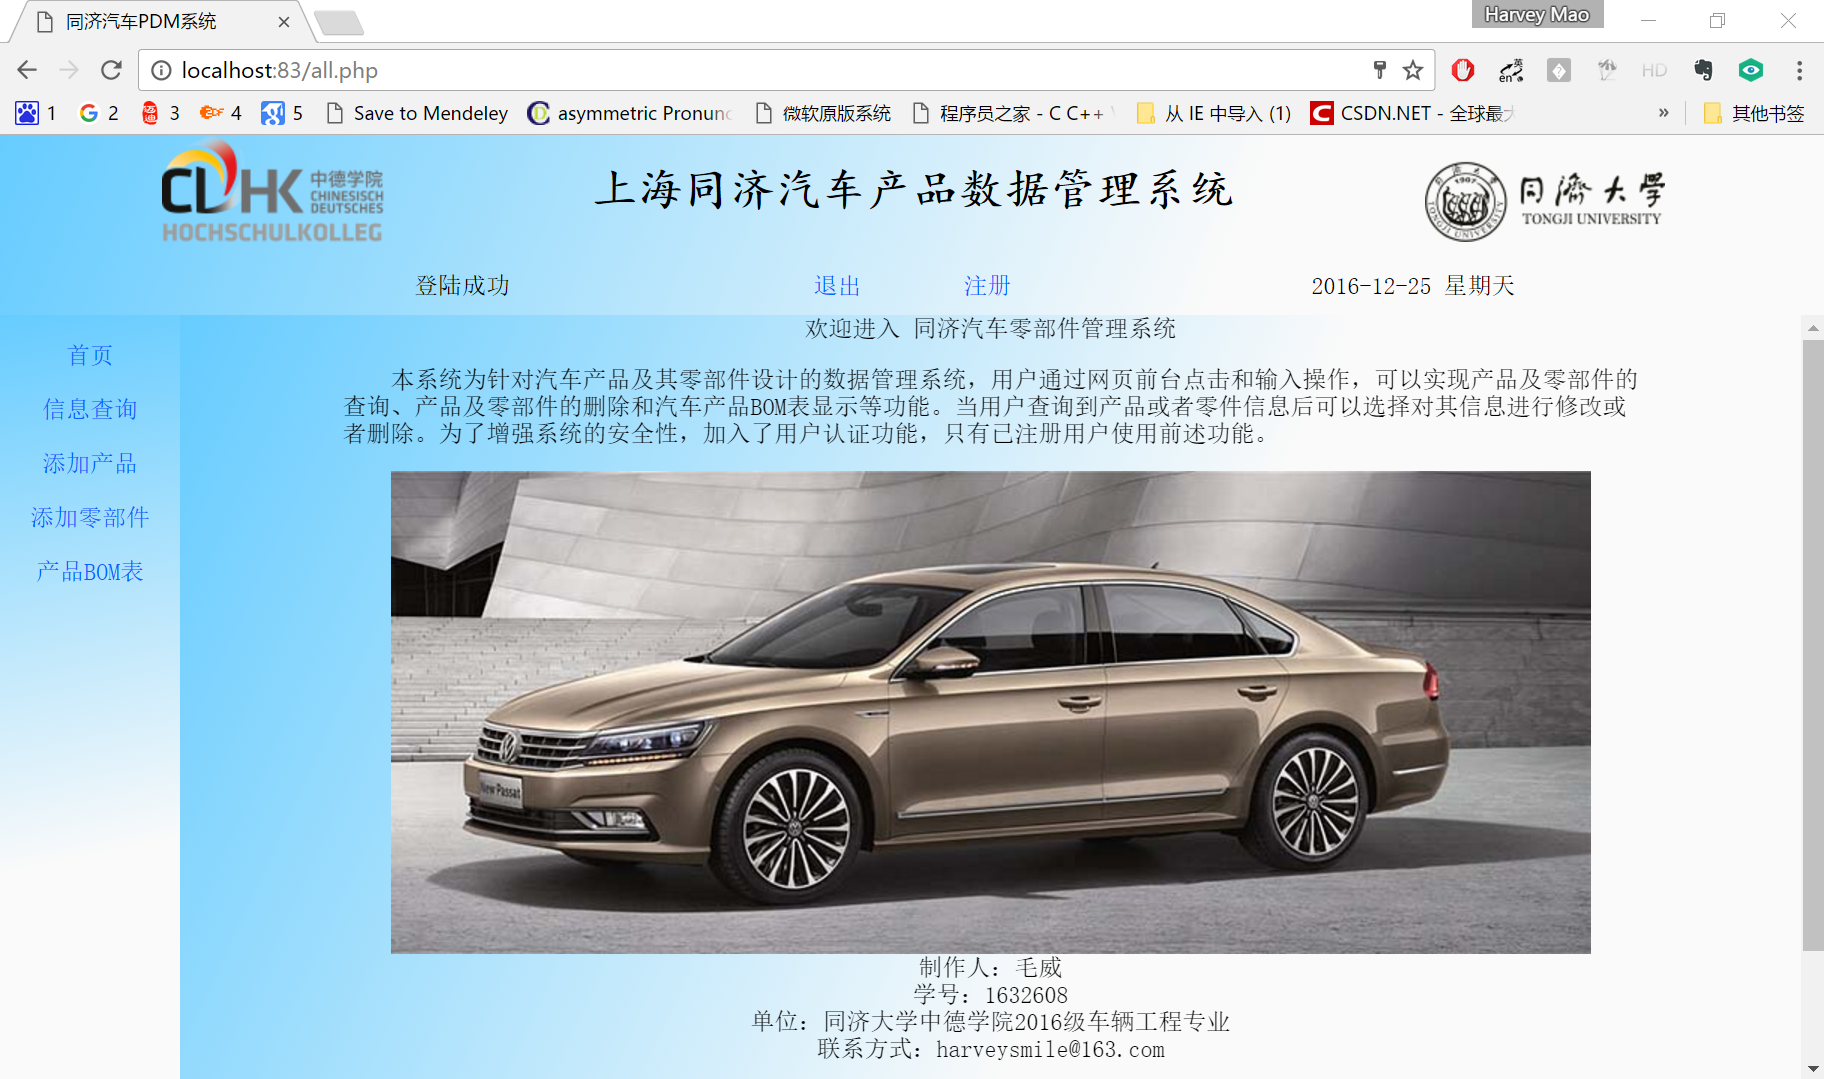
\includegraphics[width=0.9\linewidth]{figure/index}
\caption{汽车PDM动态网页}
\label{fig:index}
\end{figure}
 
站点文件结如图\ref{fig:webSite}下:
\begin{figure}[H]
\centering
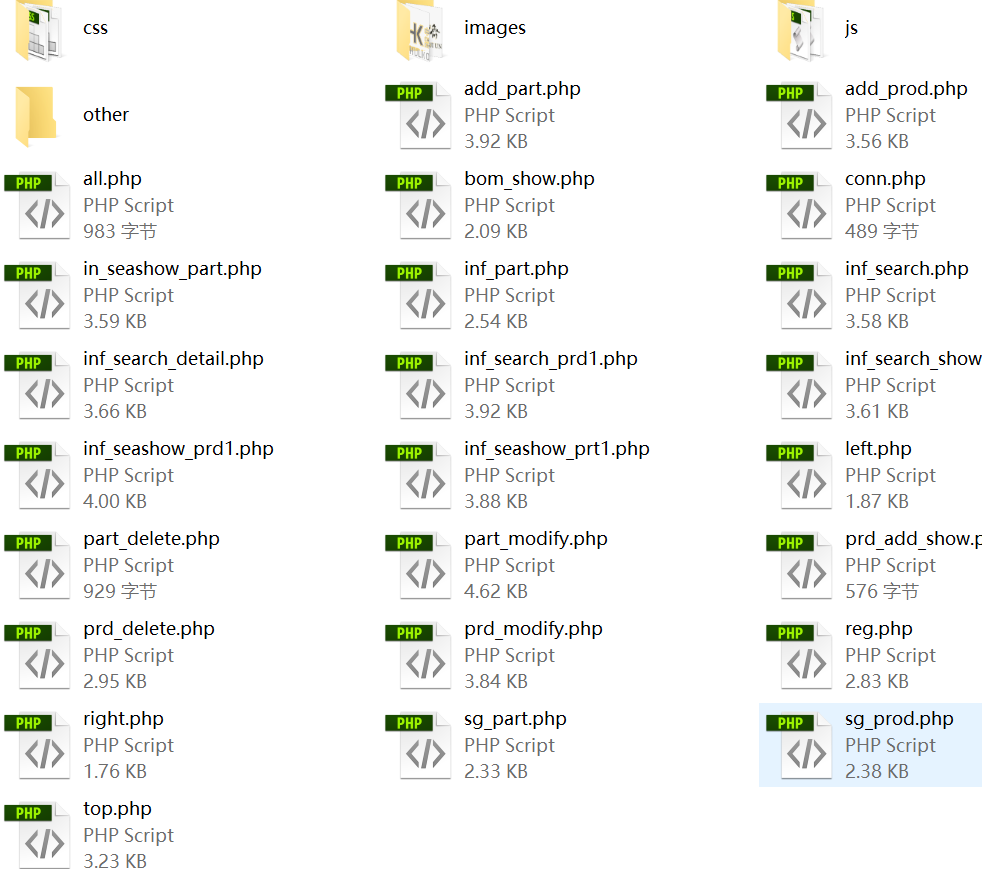
\includegraphics[width=0.8\linewidth]{figure/webSite}
\caption{汽车PDM站点}
\label{fig:webSite}
\end{figure}
